\documentclass[10pt]{beamer}
\usetheme[
%%% option passed to the outer theme
%    progressstyle=fixedCircCnt,   % fixedCircCnt, movingCircCnt (moving is deault)
  ]{Feather}


% Vorstellung / Themenbegründung
% Am Anfang Begriffsklärung

% Jahreszahlen nur letzte Folie
% Symantec Diagramm nach Unterscheidung
% Schrödingers Backup
% Nicht wiederhestellbares Backup zu Krankenhaus
% Dettelbach raus

% Quellen


% If you want to change the colors of the various elements in the theme, edit and uncomment the following lines

% Change the bar colors:
%\setbeamercolor{Feather}{fg=red!20,bg=red}

% Change the color of the structural elements:
%\setbeamercolor{structure}{fg=red}

% Change the frame title text color:
%\setbeamercolor{frametitle}{fg=blue}

% Change the normal text color background:
%\setbeamercolor{normal text}{fg=black,bg=gray!10}

%-------------------------------------------------------
% INCLUDE PACKAGES
%-------------------------------------------------------

\usepackage[utf8]{inputenc}
\usepackage[ngerman]{babel}
\usepackage[T1]{fontenc}
\usepackage{helvet}
\usepackage{eurosym}

%-------------------------------------------------------
% DEFFINING AND REDEFINING COMMANDS
%-------------------------------------------------------

% colored hyperlinks
\newcommand{\chref}[2]{
  \href{#1}{{\usebeamercolor[bg]{Feather}#2}}
}

%-------------------------------------------------------
% INFORMATION IN THE TITLE PAGE
%-------------------------------------------------------

\title[] % [] is optional - is placed on the bottom of the sidebar on every slide
{ % is placed on the title page
      \textbf{Ransomware}
}

%\subtitle[Ransomware]{Never gonna give you up}
\subtitle[Ransomware]{Yesterday - All my troubles seemed so far away}

\author[S. Abwandner, M. Beham, P. Schmid]
{      Sebastian Abwandner, Michael Beham, Pascal Schmid
}

\institute[]
{
      Hochschule Augsburg  \\
      University of Applied Sciences Augsburg
}

\date{\today}

%-------------------------------------------------------
% THE BODY OF THE PRESENTATION
%-------------------------------------------------------

\begin{document}

%-------------------------------------------------------
% THE TITLEPAGE
%-------------------------------------------------------

{\1% % this is the name of the PDF file for the background
\begin{frame}[plain,noframenumbering] % the plain option removes the header from the title page, noframenumbering removes the numbering of this frame only
  \titlepage % call the title page information from above
\end{frame}}


\begin{frame}{Gliederung}{}
\tableofcontents
\end{frame}

%-------------------------------------------------------
\section{Kleine Viren-Kunde}
%-------------------------------------------------------
\begin{frame}{Kleine Viren-Kunde}
%-------------------------------------------------------
	\begin{figure}[p]
		\centering
		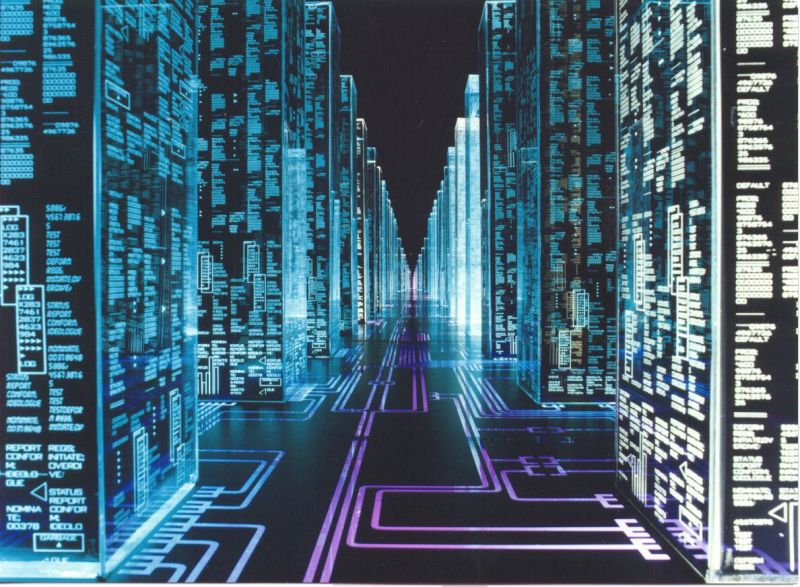
\includegraphics[scale=0.3]{hackers_internet.jpg}
		\let\thefootnote\relax\footnote{https://hackadaycom.files.wordpress.com/2013/03/hackers\_internet.jpg}
	\end{figure}
\end{frame}

\begin{frame}{Kleine Viren-Kunde}{Wer verwendet Viren?}
%-------------------------------------------------------
\begin{itemize}
	\item Security Researcher
	\item Anonymous
	\item Extremisten
	\item Regierungen (Bundestrojaner, Stuxnet)
	\item Sonstige Kriminelle
	\item Scriptkiddies
\end{itemize}
\end{frame}

\begin{frame}{Kleine Viren-Kunde}{Arten von Viren}
%-------------------------------------------------------
\begin{itemize}
	\item Viren, Würmer, Trojaner
	\item Bots, Botnetze
	\item Scareware, Ransomware
	\note{Scareware: Beheben der Gefärdungen erfordert Vollversion}
\end{itemize}
\end{frame}



%\begin{frame}{Kleine Viren-Kunde}{DOS-Viren}
%	\begin{figure}[p]
%		\centering
%		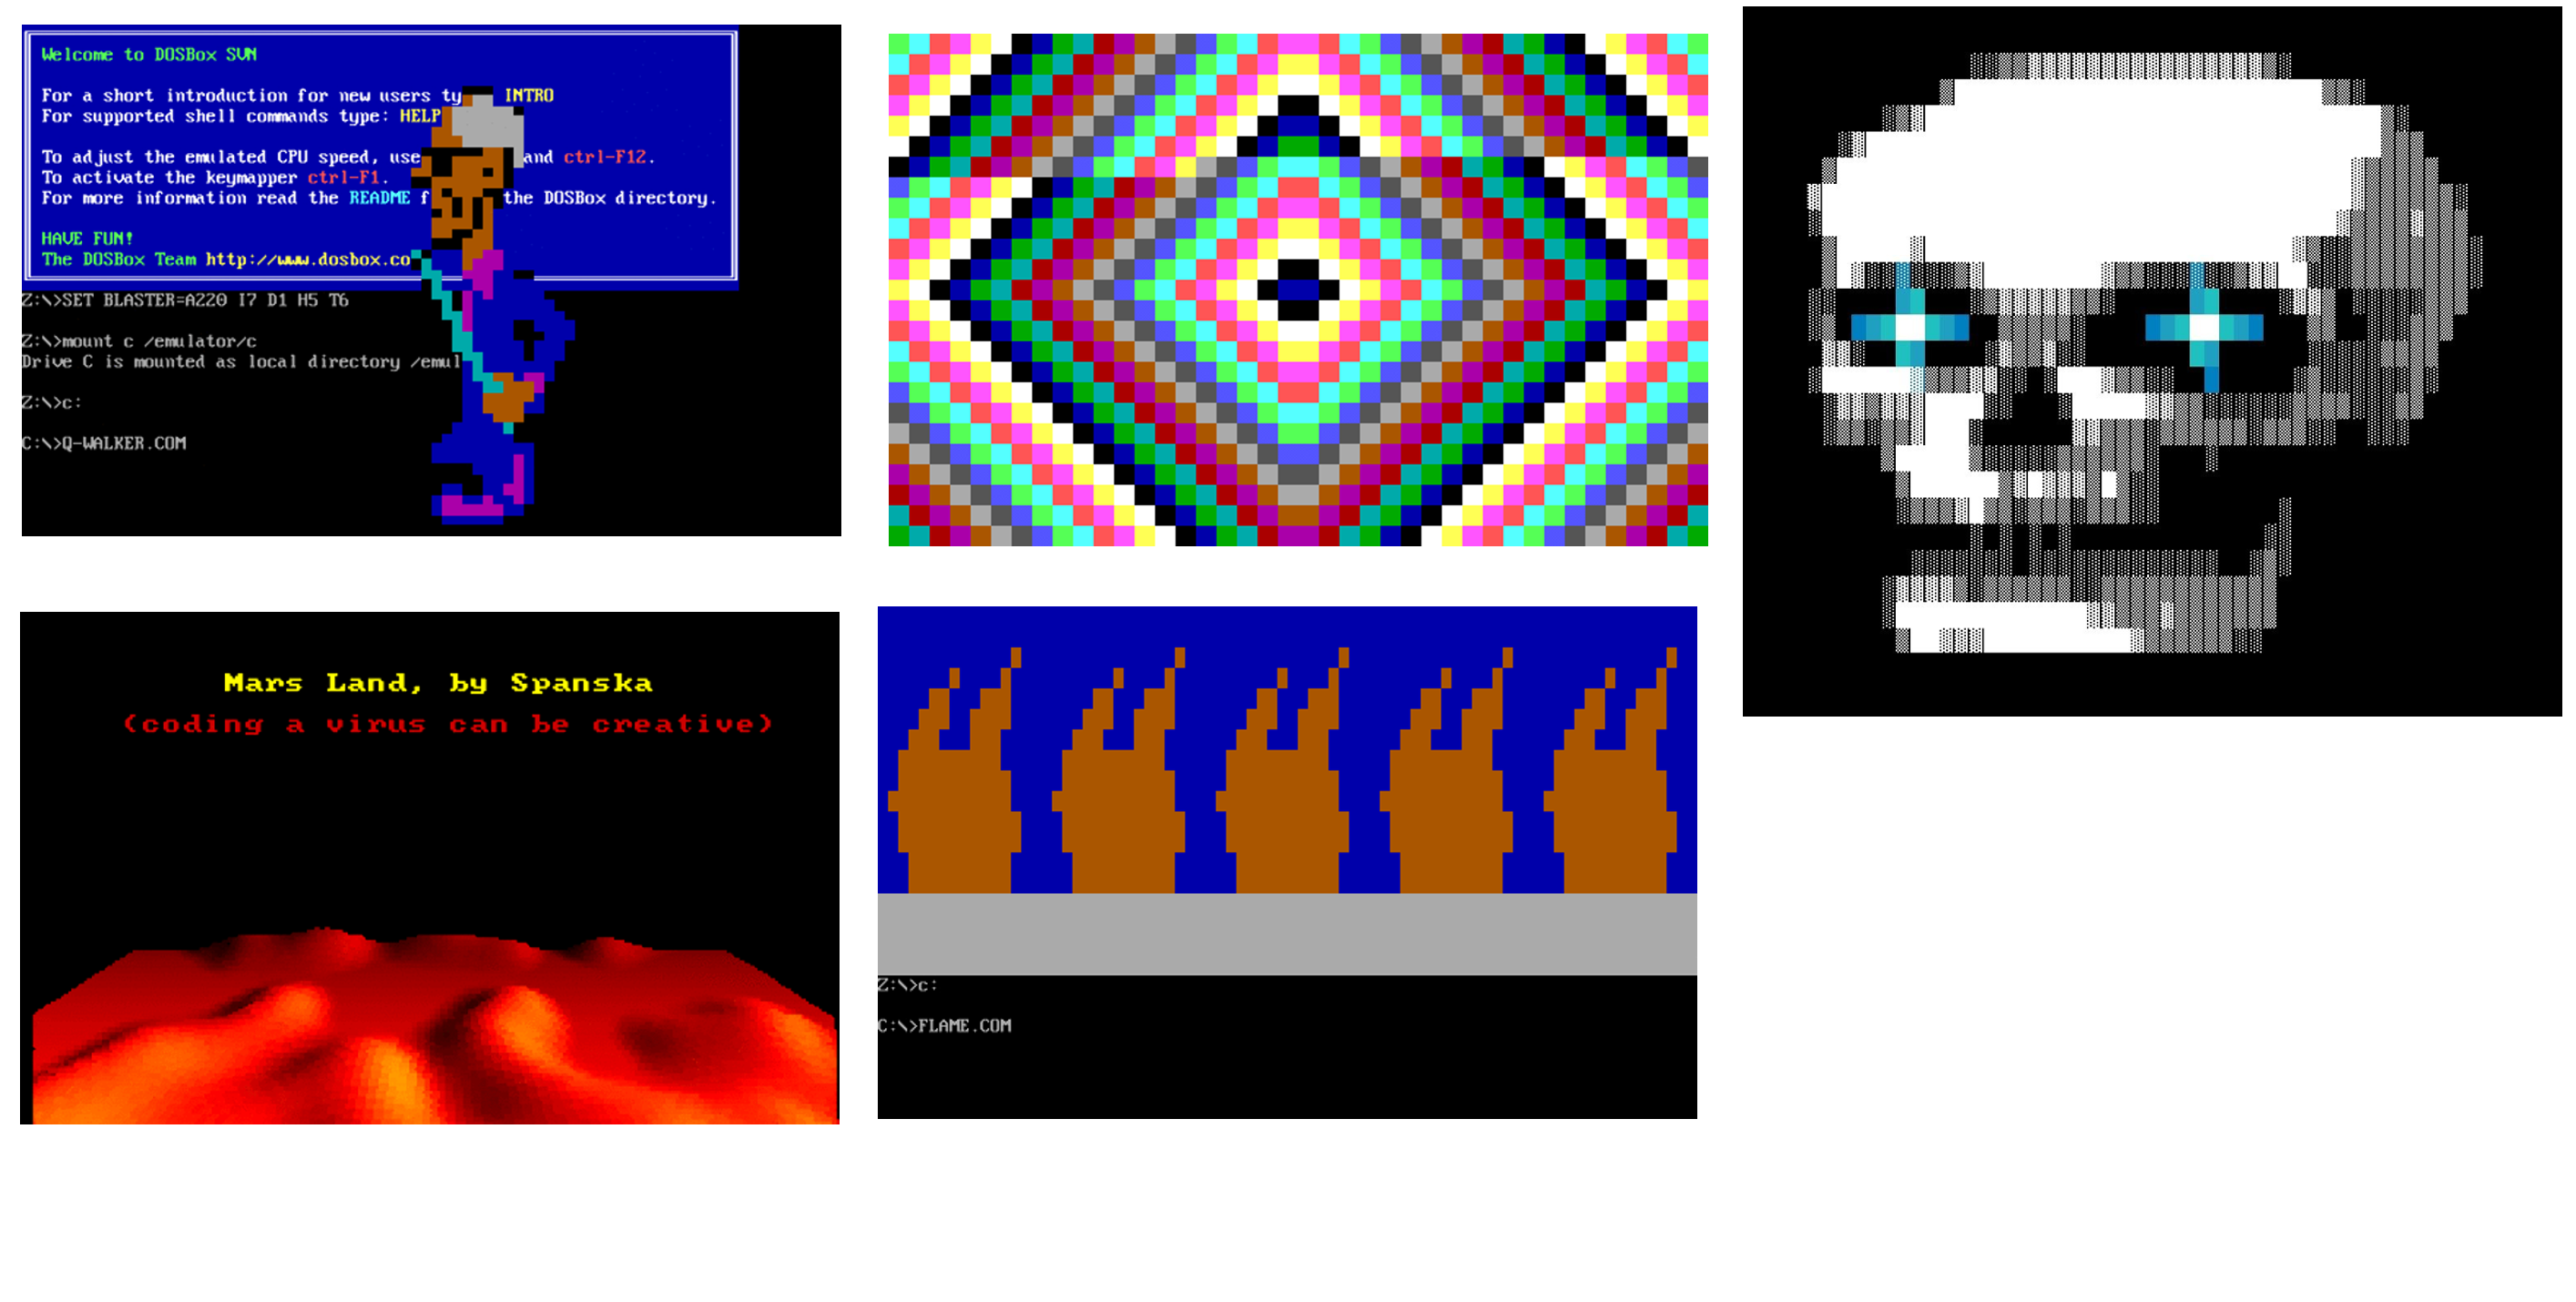
\includegraphics[scale=0.11]{dos_viruses.png}
%		\let\thefootnote\relax\footnote{\url{https://archive.org/details/malwaremuseum}}
%	\end{figure}
%\end{frame}


%\begin{frame}{Kleine Viren-Kunde}{Botnetze}
%	\begin{itemize}
%		\item Massenhaft übernommene Computer
%		\item Alle Platformen
%		\item Kapazität wird vom Botnetz-Betreiber vermietet
%	\end{itemize}
%\end{frame}


\begin{frame}{Kleine Viren-Kunde}{Ransomware}
%-------------------------------------------------------

	\begin{figure}[p]
		\centering
		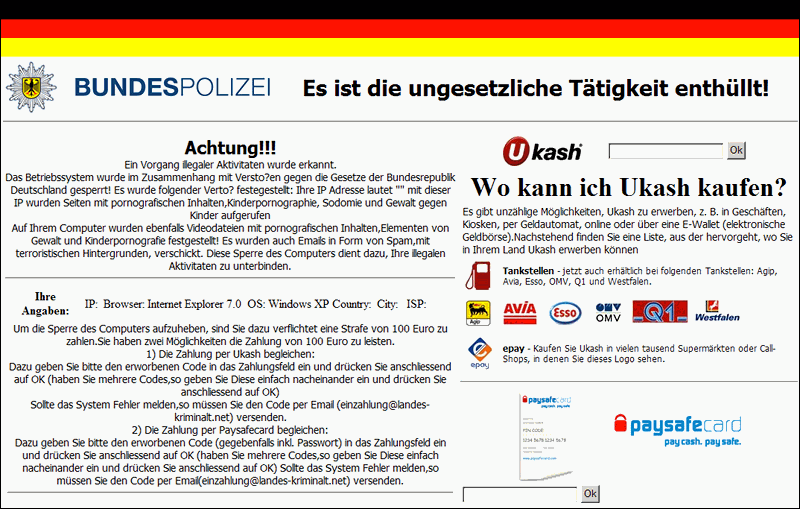
\includegraphics[scale=0.25]{bka-trojaner.png}
		\let\thefootnote\relax\footnote{\url{http://bka-trojaner.de/screenshots/bka-trojaner2.png}}
	\end{figure}

\end{frame}

\begin{frame}{Kleine Viren-Kunde}{Ransomware}
%-------------------------------------------------------
	% Siehe Liste weiter unten. Evtl. Liste nach hier
	\begin{block}{Locker Ransomware}
	\note{- Locker Ransomware spielt mit dem Vertrauen der unbedarften Anwender in die Gesetzeshüter bzw. der Angst vor Bestrafung\\}
	\note{Von den 12 meistbefallennen Ländern sind 11 davon G20-Staaten - also Staaten mit verhältnismäßig reichen Einwohnern. Die Chance diese zum Bezahlen zu bewegen sind relativ groß.\\}
		\begin{itemize}
			\item FBI, BKA, Bundespolizei, ...
			\item Entfernen leicht möglich, da kein Schaden
			\item Was bringt Zukunft?
			\note{- Bei IoT z.B. ist Interaktion nicht/kaum möglich\\}
			\note{- Was ist mit autonomen Autos?\\}
	   	\end{itemize}
	   	\note{- Locker Ransomware war nur für Heimanwender brauchbar. Admins wussten sich dagegen zu wehren\\}
	\end{block}
 	\begin{block}{Crypto Ransomware}
	  	\begin{itemize}
			\item Nutzer hat Schaden
			\item Entfernen schwierig
	   	\end{itemize}
  	\end{block}

\end{frame}


\begin{frame}{Kleine Viren-Kunde}{Geschichte der Ransomware}
%-------------------------------------------------------
	\begin{itemize}
		\item 1989: AIDS
		\item 2013: CryptoLocker (Windows)
		%\note[item]<2>{\textbf{Cryptolocker:}}
		%\note[item]<2>{(40\% aller Betroffenen zahlten}
		%\note[item]<2>{insgesamt ca. 3 Millionen \$}
		%\note[item]<2>{scannt Netzlaufwerke und angeschlossene USB-Geräte, ...)}
		\item 2013: FBI ransomware (OS X)
		\item 2014: Simplocker (Android)
		\item 2014: Oleg Pliss (iOS) (Locker Ransomware)
		\item 2016: Locky (Windows)
		\item 2016: KeRanger (OS X)
		\item 2016: Petya (Windows)
	\end{itemize}
\end{frame}


\begin{frame}{Kleine Viren-Kunde}{AIDS}
%-------------------------------------------------------
	\begin{figure}[p]
		\begin{itemize}
			\item Ransomware \textbf{AIDS} (1989)
			\item Programm mit Informationen über HIV/AIDS Ansteckung
			\item Weitergabe als legitimes Programm per Diskette \pause
			\item Kosten und Vorgehen in EULA genannt
			\item Nach dem 90. Boot: \\ Verschlüsselung aller Daten auf der Systemfestplatte
			\item Aufforderung ca. \EUR{170} an ein Postfach in Panama zu senden \pause
			\item Wissenschaftliche Arbeit mit Verbesserungsvorschlägen \\
				Yount/Yung: Cryptovirology: Extortion-Based Security Threads and Countermeasures
		\end{itemize}
		\let\thefootnote\relax\footnote{Quelle: c't Magazin 07/2016 S.77}
	\end{figure}
\end{frame}


\begin{frame}{Kleine Viren-Kunde}{Evolution der Ransomware}
%-------------------------------------------------------
	\begin{figure}[p]
		\centering
		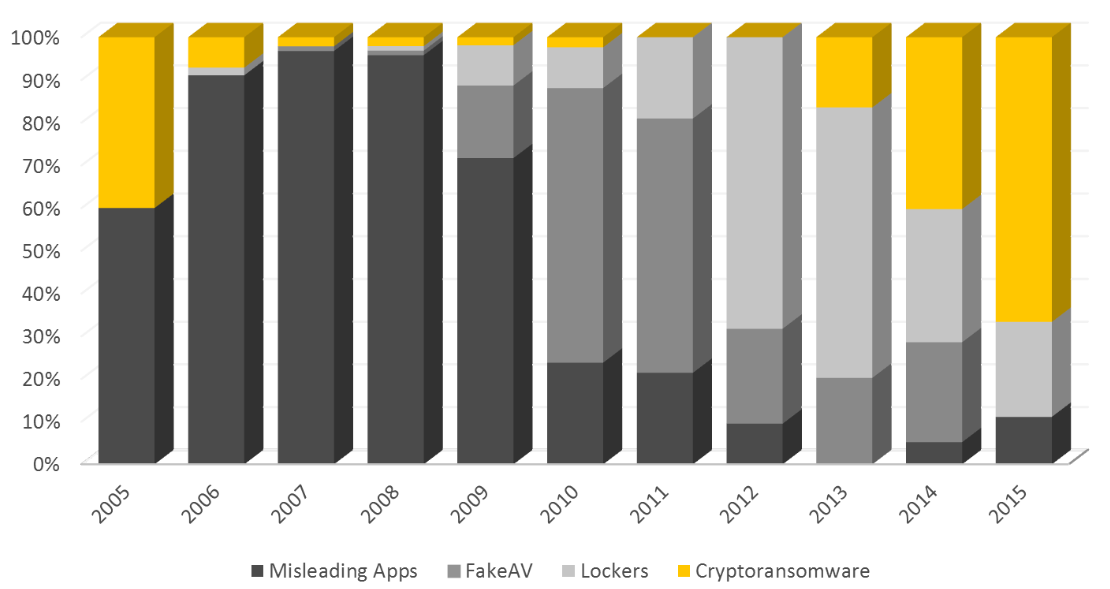
\includegraphics[scale=0.28]{ransom-evolution.png}
		\let\thefootnote\relax\footnote{\url{https://www.symantec.com/content/en/us/enterprise/media/security\_response/whitepapers/the-evolution-of-ransomware.pdf}}
		\note{Wegen schlechter anonymer internationaler Zahlungsmöglichkeit ist Anzahl von Ransomware bis zum Erscheinen von Bitcoin zurück gegangen}
	\end{figure}
\end{frame}

%\begin{frame}{Ransomware - Zeitliche Entwicklung}
%	\begin{figure}[p]
%		\centering
%		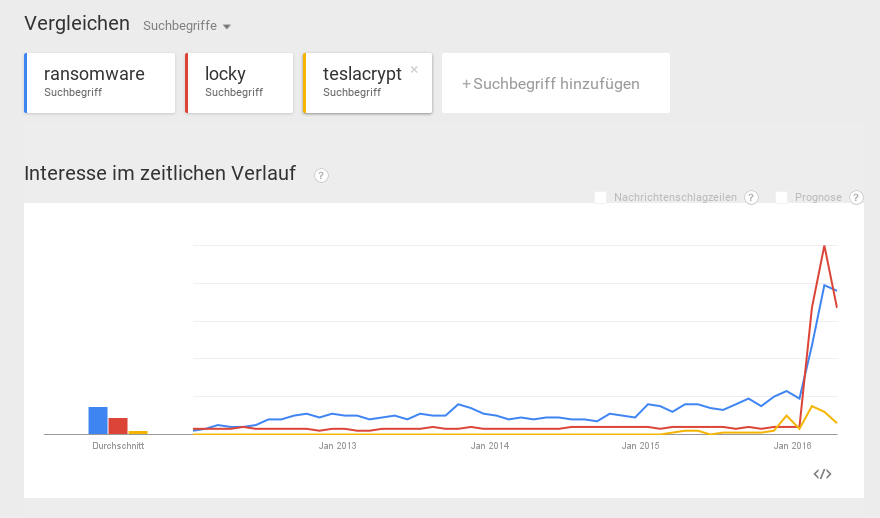
\includegraphics[scale=0.37]{ransomware_zeitablauf.png}
%	\end{figure}
%\end{frame}

\begin{frame}{Ransomware - Verteilung auf Länder}
	\begin{figure}[p]
		\centering
		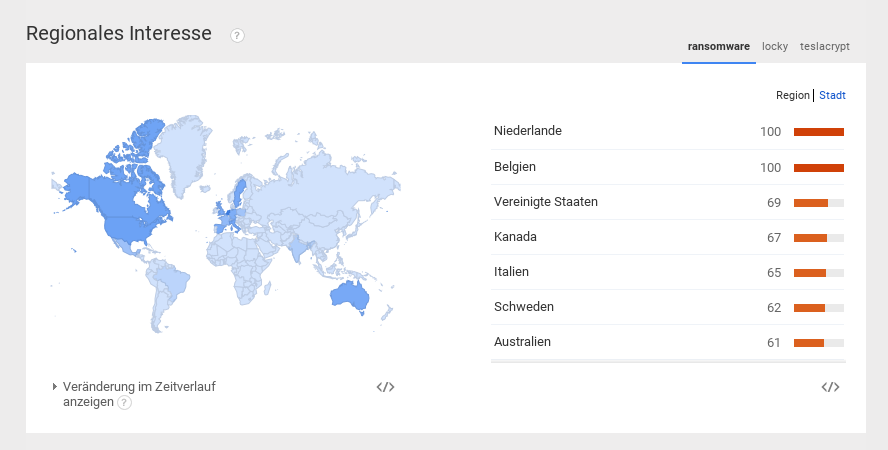
\includegraphics[scale=0.37]{ransomware_laenderverteilung.png}
	\end{figure}
\end{frame}


%-------------------------------------------------------
\section{Ransomware}
%-------------------------------------------------------
\subsection{Aktuelle Beispiele}
%\begin{frame}{Dettelbach}
%-------------------------------------------------------
%	\begin{itemize}
%		\item Stadtverwaltung von Dettelbach (Unterfranken)
%		\item Server mit "`Tesla-Crypt"' infiziert
%		\item Infektion wahrscheinlich per E-Mail-Anhang
%		\item Backups vorhanden\pause , aber nicht wiederherstellbar
%		\item Nach Zahlung von ca. \EUR{490} konnten große Teile der Daten entschlüsselt werden
%	\end{itemize}

%	\let\thefootnote\relax\footnote{\url{https://www.polizei.bayern.de/unterfranken/news/presse/aktuell/index.html/237562}}
%\end{frame}
%\begin{frame}[plain]
%	\begin{figure}[p]
%		\centering
%		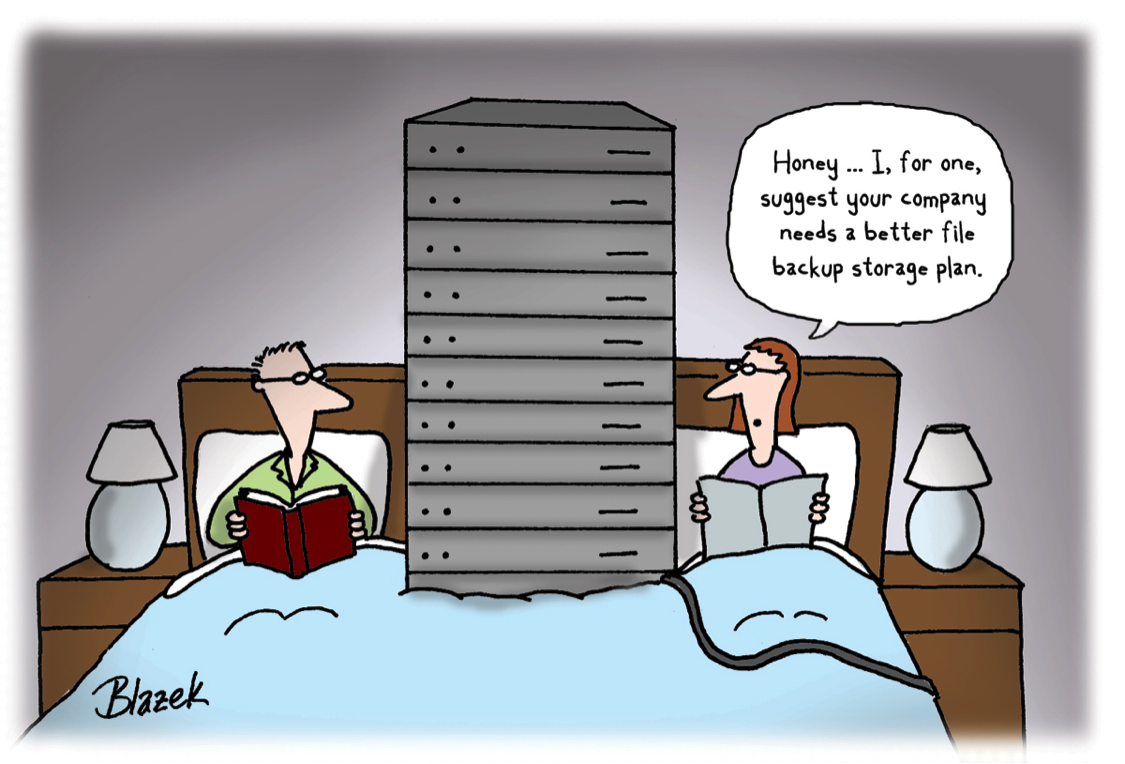
\includegraphics[scale=0.55]{backup_cartoon.png}
%		\let\thefootnote\relax\footnote{\url{http://www.evolveip.net/wp-content/uploads/2015/11/cartoon.png}}
%	\end{figure}
%\end{frame}

\begin{frame}{Lukaskrankenhaus Neuss}
%-------------------------------------------------------
	\begin{columns}
		\begin{column}{6cm}		
			\begin{itemize}
				\item Infektion per E-Mail-Anhang
				\item Sofortmaßnahme: Abschalten aller Dienste und Server (intern und extern)
				\item Organisation mit Formularen auf Papier (Notfallplan vorhanden)
				\item Aktuelles Backup vorhanden, und auch wiederherstellbar
			\end{itemize}
		\end{column}
		\begin{column}{5cm}
			\begin{figure}[p]
				\centering
				
\includegraphics[scale=0.5]{lukaskrankenhaus.jpg}
			\end{figure}
		\end{column}
	\end{columns}
	\let\thefootnote\relax\footnote{\url{http://www1.wdr.de/cyberangriff-lukaskrankenhaus-neuss-100.html}}
\end{frame}

\begin{frame}{Malvertising der BBC}
	\begin{columns}
		\begin{column}{6cm}
			\begin{itemize}
				\item Webseiten wurden gezielt attackiert
				\item Opfer der Kampagne: New York Times, BBC, AOL, NFL
				\item Advertisments wurden gekapert
				\item Funktioniert dank Browser Betriebssystem-unabhängig
			\end{itemize}
		\end{column}
		\begin{column}{5cm}
			\begin{figure}[p]
				\centering
				
\includegraphics[scale=0.1]{BBC.png}
			\end{figure}
		\end{column}
	\end{columns}
	\let\thefootnote\relax\footnote{\url{http://www.theguardian.com/technology/2016/mar/16/major-sites-new-york-times-bbc-ransomware-malvertising}}
\end{frame}


\begin{frame}{Faktoren von Ransomware}
%-------------------------------------------------------

	\begin{itemize}
		\item Ökonomie
		\item Psychologie
		\item Social-Engineering
		\note{- Crypto Ransomware zeigt oft einen Countdown, bis zu dem die Nutzer bezahlt haben müssen, um dem Verlust ihrer Daten vorzubeugen. So wird ein Einschreiten von Admins oder Polizei verhindert}
		\note{- Landesabhängiger Preis für Wiedererhalt der Daten je nach Kaufkraft des Landes - basierend auf IP-Adresse}
			\note{- Crypto wird mit BTC bezahlt, während Locker eher auf Paysafecard und ähnliches aus dem Laden zurückgreift. Dies hat die Ursache darin, dass der Computer ja gesperrt ist und nicht zum BTC kaufen genutzt werden kann.\\}
		\note{- BTC wird in Videos erklärt und wie der Nutzer sie kaufen und verwenden kann.\\}
		\note{- Manche Ransomware erlaubt es 5 zufällige Dateien zu entschlüsseln, um dem Nutzer zu zeigen, dass es mit Bezahlung möglich ist.}
	\end{itemize}
\end{frame}

\begin{frame}{Faktoren von Ransomware}{Locker Ransomware}
%-------------------------------------------------------
\begin{columns}
\begin{column}{6cm}
\textbf{Zentrale und periphere Route zur Überzeugung}
\begin{itemize}
\item \textbf{Zentral:} Vorsichtige und durchdachte Abwägung der Vorzüge
\item \textbf{Peripher:} Positive/Negative Konnotation mit Worten
\end{itemize}
\end{column}
\begin{column}{5cm}
\begin{figure}[p]
		\centering
		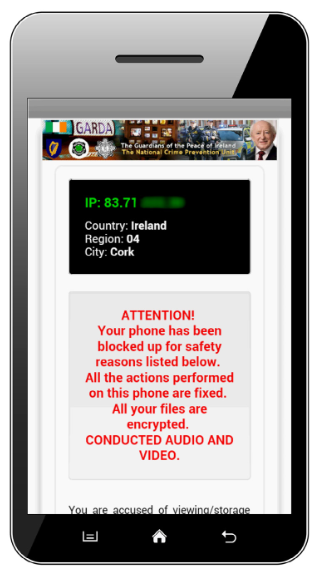
\includegraphics[scale=0.3]{Lockdroid.png}

	\end{figure}
\end{column}
\end{columns}

	\let\thefootnote\relax\footnote{\url{https://www.symantec.com/content/en/us/enterprise/media/security\_response/whitepapers/the-evolution-of-ransomware.pdf}}
	\note{\textbf{Locker Ransomware}\\}
	\note{- Befolgen von Authoritäten\\}
	\note{- Instinktive Trigger dank IP-Adresse (Furcht)\\}
	\note{- If you have broken the law, it can be used against you
. Furcht wegen illegalen Downloads um Hilfe zu bitten.\\}
	\note{- Wenn Opfer nach der Errornachricht suchen, sehen sie eher die rechtliche Legitimität als deren erfundene Gestalt. Vor allem da die meisten Menschen mit den präsentierten Gesetzestexten nichts anfangen können.\\}
\end{frame}

\begin{frame}{Faktoren von Ransomware}{Crypto Ransomware}
%-------------------------------------------------------

	\begin{figure}[p]
		\centering
		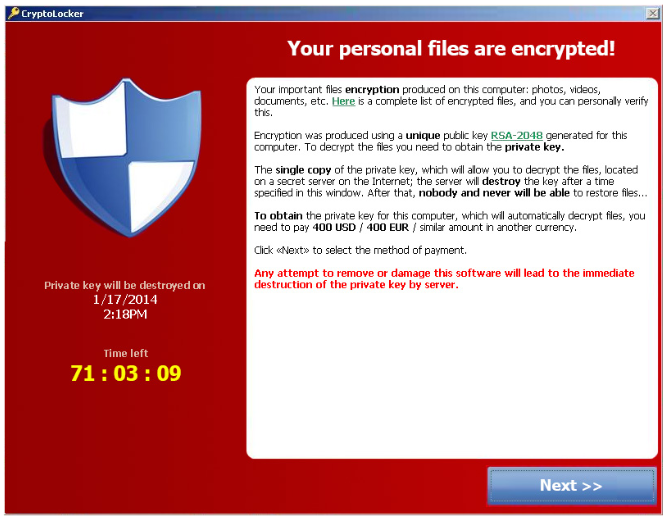
\includegraphics[scale=0.33]{Cryptolocker.png}
	\end{figure}

	\let\thefootnote\relax\footnote{\url{https://www.symantec.com/content/en/us/enterprise/media/security\_response/whitepapers/the-evolution-of-ransomware.pdf}}
	\note{\textbf{Crypto Ransomware}\\}
	\note{- Timeout setzt Entscheidungsfindung unter Druck\\}
	\note{- Sunk costs: Bereits getätigtes Investment (Zeit/Geld) wird aufgerechnet und wirkt, dass das Scamopfer zahlt.\\}
	\note{- Furcht vor Gewissensbissen, falls sie nicht zahlen.\\}
	\note{- \textbf{Ellsberg-Paradoxon:} Eine Strafe mit sicherer Wahrscheinlichkeit wird eher gewählt, als ein positives Ergebnis mit unsicherer Wahrscheinlichkeit.\\}

\end{frame}

\section{Kryptographie}
\subsection{Symmetrische Verschlüsselung}
\begin{frame}{Kryptographie}{Symmetrische Verschlüsselung}
	\begin{columns}
		\begin{column}{6cm}
			\textbf{Symmetrische Verschlüsselung}
			\begin{itemize}
				\item Gleicher Schlüssel für Ver- und Entschlüsselung
				\item Typischer Vertreter: \textbf{AES} (Advanced Encryption Standard)
				\item Schneller Algorithmus mit Prozessorunterstützung
				\item Geeignet auch für große Datenmengen
			\end{itemize}
		\end{column}
		\begin{column}{5cm}
			\begin{figure}[p]
				\centering
				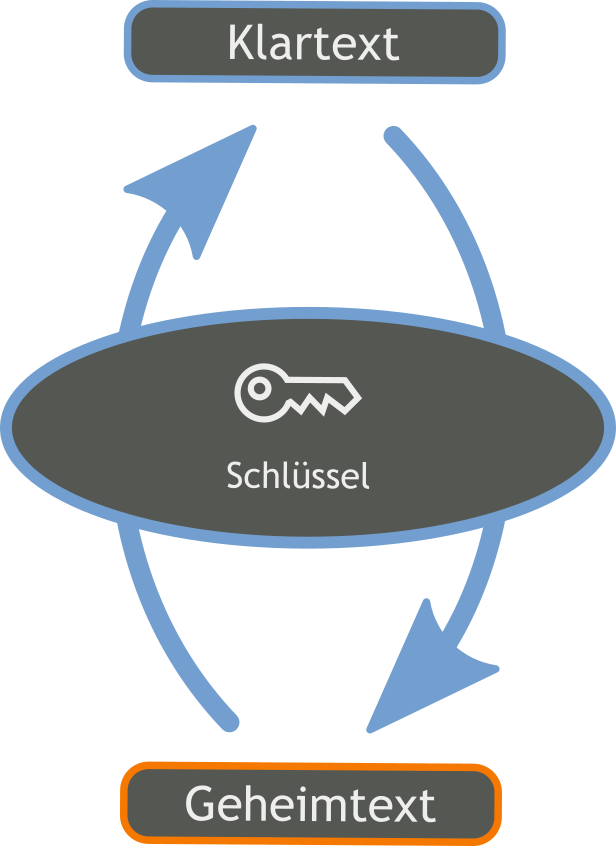
\includegraphics[scale=0.25]{SymKrypto.png}
			\end{figure}
		\end{column}
	\end{columns}
	\let\thefootnote\relax\footnote{Nach \url{https://commons.wikimedia.org/wiki/File:Orange_blue_symmetric_cryptography_de.svg}}
	\note{\textbf{Symmetrische Verschlüsselung}\\}
	\note{- \\}
	\note{- Sunk costs: Bereits getätigtes Investment (Zeit/Geld) wird aufgerechnet und wirkt, dass das Scamopfer zahlt.\\}
	\note{- Furcht vor Gewissensbissen, falls sie nicht zahlen.\\}
	\note{- Hohe Geschwindigkeit: Modere Prozessoren \\}

\end{frame}

\subsection{Asymmetrische Verschlüsselung}
\begin{frame}{Kryptographie}{Asymmetrische Verschlüsselung}


	\begin{columns}
		\begin{column}{6cm}
			\textbf{Asymmetrische Verschlüsselung}
			\begin{itemize}
				\item Zwei Schlüssel: Verschlüsselung und Entschlüsselung (Privat / Öffentlich)
				\item Mathematisch sicher bei großer Schlüssellänge (> 2048 Bit)
				\item Hoher Rechenaufwand, daher nicht für große Datenmenge geeignet
			\end{itemize}
		\end{column}
		\begin{column}{5cm}
			\begin{figure}[p]
				\centering
				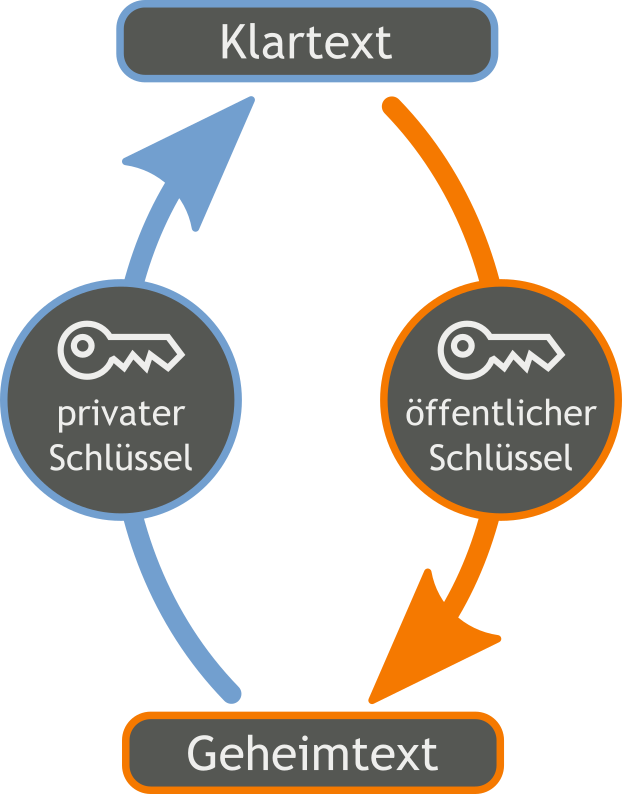
\includegraphics[scale=0.25]{AsymKrypto.png}
			\end{figure}
		\end{column}
	\end{columns}
	\let\thefootnote\relax\footnote{Nach \url{https://commons.wikimedia.org/wiki/File:Orange_blue_public_key_cryptography_de.svg}}
\end{frame}

\subsection{Hybride Verschlüsselung}
%\begin{frame}{Hybride Verschlüsselung}
%	\begin{itemize}
%		\item Sitzungsschlüssel zufällig erzeugen
%		\item Sitzungsschlüssel für AES verwenden
%		\item Sitzungsschlüssel asymmetrisch verschlüsseln
%	\end{itemize}
%\end{frame}
\begin{frame}{Kryptographie}{Hybride Verschlüsselung}
	\begin{figure}[]
		\centering
		%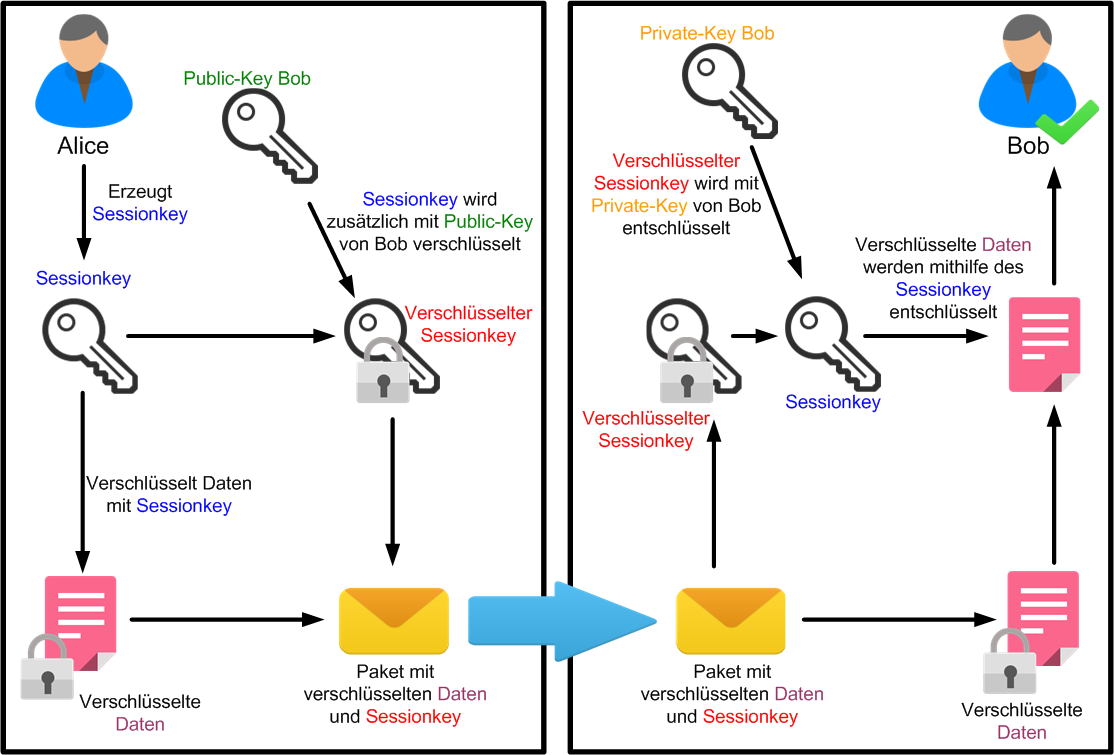
\includegraphics[scale=0.25]{hybrid.png}
		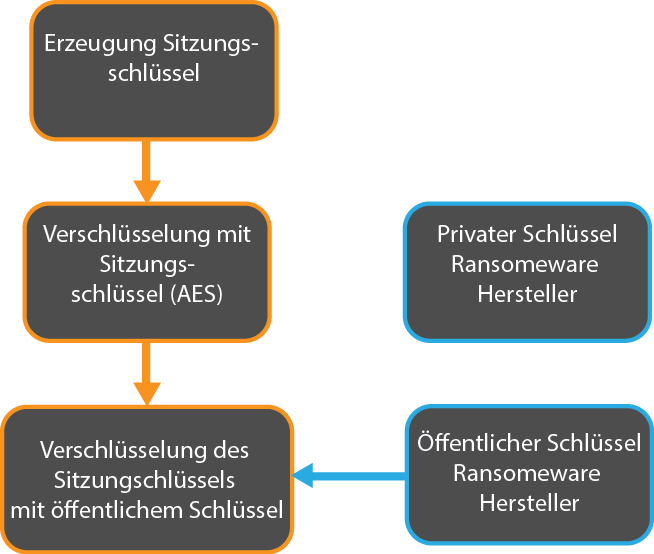
\includegraphics[width=.6\linewidth]{hybride_Verschluesselubg.png}
	\end{figure}
\end{frame}
% https://de.wikipedia.org/wiki/Datei:Hybride_Verschl%C3%BCsselung.png



\subsection{Funktionsweise}
\begin{frame}{Ransomware}{Infektion}
		\begin{itemize}
			\item weite Streuung
			\item meist unspezifisch
			\item Verbreitungswege:
				\begin{itemize}
					\item E-Mail
					\item Webseiten (Drive-By-Downloads, Wordpress)
					\item Makros (Excel, Word)
				\end{itemize}
			\item Umgehen der Heuristiken von Virenscannern (Warten)
			\item RaaS: Ransomware as a Service
		\end{itemize}
\end{frame}
\begin{frame}{Ransomware}{Angriff}
		\begin{itemize}
			\item C2-Server finden und kontaktieren
			\item Asym. Schlüssel erstellen (Öffentlich und Privat)
			\item Privaten Schlüssel an Server senden und lokal vernichten
			\item Dateien hybrid verschlüsseln 
		\end{itemize}
		\note{Asym. Schlüssel evtl. auch von Server / DoS Möglichkeit}
\end{frame}

\begin{frame}[plain]
	\begin{figure}[p]
		\centering
		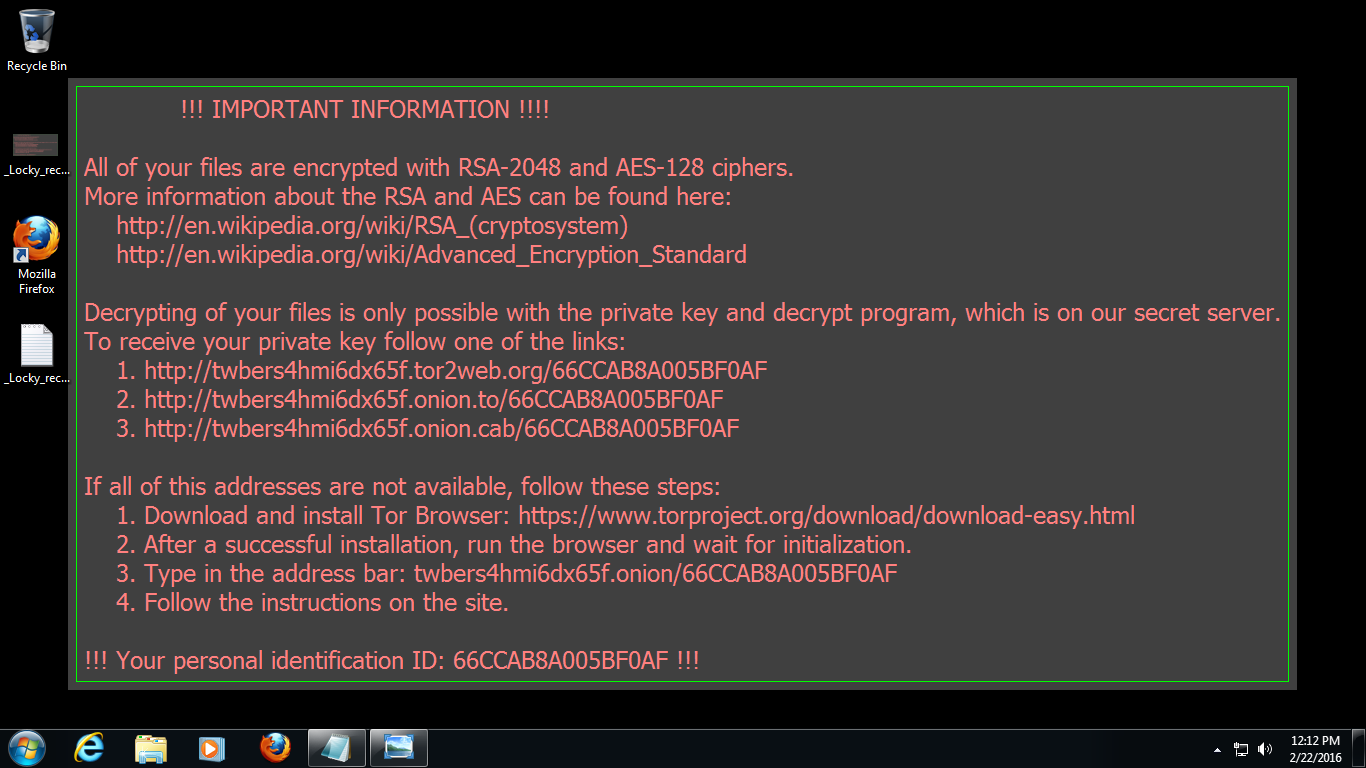
\includegraphics[scale=0.30]{locky-recover-instructions.png}
		\let\thefootnote\relax\footnote{\url{https://labsblog.f-secure.com/2016/02/22/locky-clearly-bad-behavior/}}
	\end{figure}
\end{frame}

\begin{frame}{Ransomware}{Bezahlung}
	\begin{itemize}
		\item Nutzer informieren
		\item Genaue Anleitung unter Onion-Adresse (Tor-Netzwerk)
		\note{Kurze Erklärung zu Tor}
		\item Bezahlung per Bitcoin
		\note{Kurze Erklärung zu Bitcoin}
		\item Meist mit Zeitlimit und Drohungen
	\end{itemize}
\end{frame}


\begin{frame}{Ransomware}
	\begin{itemize}
		\item Wenn Bezahlung an Adresse eingegangen ist ...
		\item bekommt man evtl. den privaten Schlüssel
		\item und kann die Dateien entschlüsseln
	\end{itemize}
	\note{Quelle notwendig, Übertragungsweg?}
\end{frame}


\subsection{Gegenmaßnahmen}
\begin{frame}{Gegenmaßnahmen}
%-------------------------------------------------------
	\begin{figure}[p]
		\centering
		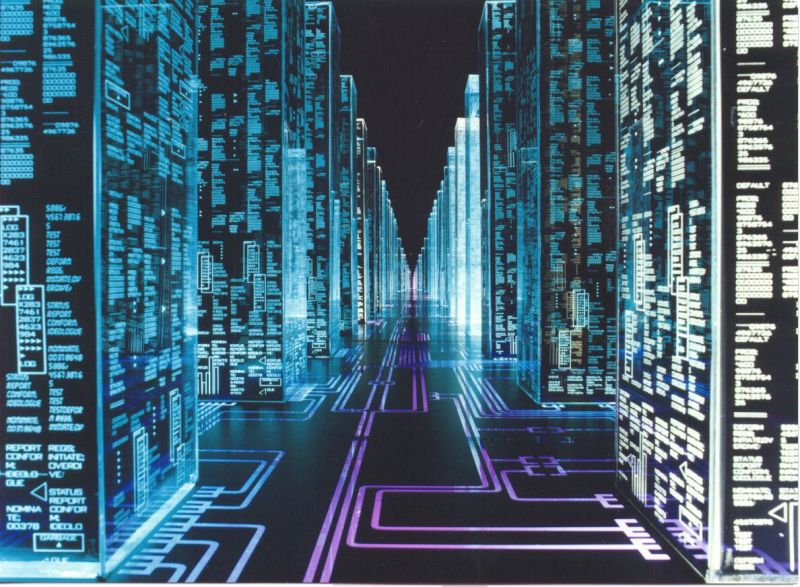
\includegraphics[scale=0.3]{hackers_internet.jpg}
		\let\thefootnote\relax\footnote{https://hackadaycom.files.wordpress.com/2013/03/hackers\_internet.jpg}
	\end{figure}
\end{frame}
\begin{frame}{Prävention}
	Nach Empfehlungen des BSI
	\begin{itemize}
		\item Aktuelle Patchlevel
		\item Angriffsfläche minimieren (Browser, Skripts im OS)
		\item Makros deaktivieren (Office etc.)
		\note{
		\item Text-Mails erzwingen
		\item Serverseitige Mailfilter
		\item Netzlaufwerke sichern
		\item Netzwerke segmentieren
		\item Zugänge sichern (RDP, Admin-Zugänge)
		\item Aktueller Virenschutz 
		\item Nutzerschulung
			\note{Nutzer sind kreativ beim Umgehen von Sicherheitsmaßnahmen (Bsp. Kennwörter)}
	\end{itemize}
	\let\thefootnote\relax\footnote{https://www.bsi.bund.de/SharedDocs/Downloads/DE/BSI/Cyber-Sicherheit/Themen/Ransomware.pdf}
\end{frame}

\begin{frame}{Schadensbegrenzung}
	\begin{itemize}
		\item Betroffene System abschotten und abschalten
		\item Kommunikation mit C2-Servern unterbinden
		\item Zentrale Ressourcen schützen (Fileserver etc.)
	\end{itemize}
\end{frame}

\begin{frame}{Notfallkonzept}
%-------------------------------------------------------
	\begin{itemize}
		\item Aktuelle Offline-Backups
		\note{Zeitabstände nach akzeptablen Verlust}
		\item Rücksicherung testen (Schrödingers Backup)
						
		\item Ersatzpläne für Systemausfälle
 	\end{itemize}

\end{frame}


{\1
\begin{frame}[plain,noframenumbering]
  \finalpage{Vielen Dank für Eure Aufmerksamkeit!}
\end{frame}}

{\1
\begin{frame}[plain,noframenumbering]
	\begin{figure}[p]
		\centering
		
\includegraphics[scale=0.1]{questionmark.png}
	\end{figure}
\end{frame}}

\end{document}
